\documentclass[tikz, border=4pt]{standalone}
\usepackage{tikz}
\usepackage{blochsphere}
\begin{document}
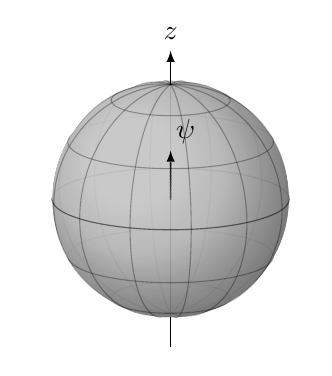
\begin{tikzpicture}[x=1cm, y=1cm]
  \node[inner sep=0pt] at (1.52,-2.08) {\pgfinterruptpicture%
  \begin{blochsphere}[radius=1.5cm, tilt=15, rotation=-20]
    \drawBallGrid[style={opacity=0.3}]{30}{30}
    \drawAxis[scale=1.3, axisarrow={->}]{0}{0}
    \labelPolar[scale=1.45]{z}{0}{0}
    \node at (z) {$z$};
    \drawStatePolar{psi}{50}{70}
    \node[above right] at (psi) {$\psi$};
  \end{blochsphere}%
  \endpgfinterruptpicture};
\end{tikzpicture}
\end{document}
